\documentclass{article}

% Language setting
\usepackage[french]{babel}

% Set page size and margins
\usepackage[letterpaper,top=2cm,bottom=2cm,left=3cm,right=3cm,marginparwidth=1.75cm]{geometry}

% Useful packages
\usepackage{amsmath}
\usepackage{graphicx}
\usepackage{hyperref}
\usepackage{float}

\title{PG4 : Akropolis}
\author{Nidhal Moussa \& Mathéo Piget \& Benzerdjeb Reyene \& Gbaguidi Nerval \& Chetouani Bilal
}
\date{\today}

\begin{document}

    \maketitle

    \tableofcontents

    \newpage

    \section{Introduction}\label{sec:introduction}

    \subsection{Présentation du Projet}\label{subsec:presentation-du-projet}
    Le projet consiste en la réalisation d'un jeu de société nommé Akropolis, qui est un jeu tour par tour dont le but est de construire une cité antique.
    Le jeu se déroule sur un plateau de jeu composé de cases hexagonales.
    Chaque joueur possède un certain nombre de ressources qu'il peut utiliser pour construire des bâtiments sur les cases du plateau.
    Chaque bâtiment rapporte des points de victoire à son propriétaire en remplissant certaines conditions.
    Il est aussi possible de les faire supperposer pour obtenir d'avantage de points.
    Il faut donc gérer le placement des bâtiments pour maximiser les points de victoire.
    La pioche de tuiles est limitée. Le jeu se termine lorsqu'il n'en reste qu'une.
    Le joueur qui a le plus de points de victoire à la fin de la partie est déclaré vainqueur.

    Réalisé en java et en utilisant la bibliothèque graphique Swing, le jeu est jouable en local sur un ordinateur.

    \subsection{Objectifs}\label{subsec:obectifs}

    L'objectif principal du projet est de réaliser un jeu de société complet et fonctionnel, avec une interface graphique permettant de jouer en local sur un ordinateur.
    Les objectifs secondaires ont été de réaliser un jeu agréable à jouer, avec une interface graphique intuitive et des graphismes de qualité.

    \section{Gestion du projet}\label{sec:gestion-du-projet}

    \subsection{Méthode}\label{subsec:methode}

    Pour la gestion du projet, nous avons opté pour une méthode de développement agile, basée sur des itérations courtes et des réunions régulières pour faire le point sur l'avancement du projet et discuter des problèmes rencontrés.
    Nous avons également utilisé un dépôt Git pour gérer les différentes versions, ce qui nous a permis de travailler en parallèle sur les différentes parties du jeu et de fusionner nos modifications facilement.
    Nous avons priviligé en priorité la réalisation du modèle de jeu en implémentant les règles du jeu.
    Nous avons ensuite travaillé sur la vue (ce qui fût la partie la plus longue) et relier le modèle à la vue en implémentant le contrôleur.

    \subsection{Répartition des taches}\label{subsec:repartition-des-taches}
    Pour la réalisation du projet, nous avons réparti les tâches en fonction des compétences de chacun.
    La polyvalence de chacun nous a permis de travailler sur plusieurs aspects du jeu.
    Nous avons également organisé des réunions régulières (plus ou moins obligatoire grâce à ce cours) pour discuter de l'avancement du projet et des problèmes rencontrés (voir section \ref{sec:difficultes-rencontrees}).

    \subsection{Architecture du Projet}\label{subsec:architecture-du-projet}
    Pour ce projet, nous avons opté pour une architecture orientée objet, avec une séparation claire entre les différentes parties du jeu, basé sur un modèle MVC (Modèle-Vue-Contrôleur) car beaucoup plus modulable et facile à maintenir, pour faire des modifications ou ajouter des fonctionnalités.
    La partie graphique du jeu est gérée par la bibliothèque Swing, qui permet de créer des interfaces graphiques en Java.
    Avec une grande partie assez abstraite, le jeu est facilement modifiable et extensible, principalement pour les jeux de société.
    \newline
    Plusieurs règles ont été mises en place pour faciliter la gestion de ce projet.
    Nous nous sommes interdit d'utiliser des bibliothèques externes pour la réalisation du jeu, à l'exception de JUnit pour les tests unitaires.
    La raison de cette interdiction est que nous ne voulious pas utiliser de build tools comme Maven ou Gradle pour gérer les dépendances.
    Elles auraient demandé à l'utilisateur de les installer pour pouvoir lancer le jeu, ce qui aurait été une contrainte supplémentaire.
    Nous avons limiter au maximum l'utilisation de variables globales.
    La raison est que cela évite les cas où un objet a été modifié dans une version précédente du code et que cela a des conséquences inattendues dans une autre partie du code.
    Nous avons essayé au maximum de profiter de l'orienté objet : chaque classe doit s'autogérer le plus possible.
    Nous avons evité d'abusé du principe de l'héritage, préférant la composition.
    L'héritage est un outil puissant mais qui peut être dangereux s'il est mal utilisé.
    La composition est souvent plus simple et plus flexible que l'héritage.
    Il est plus facile de changer le comportement d'un objet en changeant les objets avec lesquels il travaille qu'en changeant sa classe mère.
    En changeant sa classe mère, on change le comportement de tous les objets de cette classe, ce qui peut avoir des conséquences inattendues.
    \newline
    En ce qui concerne les noms des variables, nous avons essayé de les rendre le plus explicite possible.
    Le cammelCase a été utilisé pour les noms de variables, de méthodes et de classes. 
    Les noms de classes commencent par une majuscule, les noms de méthodes et de variables par une minuscule.
    Les noms de classes sont des noms qui décrivent en quoi consiste la classe.
    Les noms de méthodes sont des verbes, les noms de variables sont des noms qui décrivent ce que contient la variable.
    On essaye de nommer nos variables en anglais. La raison est que c'est la convention la plus utilisée dans le monde de la programmation.
    De plus, si on travaille sur un projet open source, il est plus facile pour les autres contributeurs de comprendre le code si les noms des variables sont en anglais.
    Cela peut paraître trivial mais cela rend le code plus lisible et plus facile à comprendre.
    Nous avons profiter au maximum de la JavaDoc pour documenter notre code.
    L'avantage de la JavaDoc est qu'elle permet de générer une documentation à partir du code source.
    En plus de cela, les IDE modernes comme IntelliJ IDEA ou Eclipse permettent de voir la JavaDoc d'une méthode ou d'une classe simplement en passant la souris dessus.
    Cela permet de voir rapidement ce que fait une méthode ou une classe sans avoir à ouvrir le fichier source.
    \newline
    Pour ce qui concerne le MVC, nous nous sommes fixé des règles dessus.
    Le modèle ne doit jamais communiquer directement avec la vue.
    Il ne doit pas contenir quelque chose qui a trait à l'interface graphique, seulement du code logique.
    Il ne peut envoyer que des informations au contrôleur ou à d'autres modèles pour lui dire ce qu'il se passe.
    Pour cela on utilise des PropertyChangeListeners qui permettent de mettre en place le pattern Observer.
    La mise en place du pattern Observer se réalisera grâce à notre classe abstraite Controller qui implémente l'interface PropertyChangeListener.
    Chaque controller extend de cette classe abstraite. Les classes du modèle en relation avec le controller extend de la classe Modèle qui contient les méthodes pour ajouter et supprimer des PropertyChangeListeners.
    Cela réduit le code redodant dans ces classes. L'intérêt de ce pattern est d'éviter une ijection directe de dépendance entre le modèle et la vue.
    On contrôle plus facilement les interactions entre les classes, savoir ce que l'on veut envoyer et recevoir ce qui facilite le débuggage puisque ces interactions sont centralisées dans la méthode propertyChange.
    Le contrôleur peut envoyer des informations à la vue pour lui dire de se mettre à jour et peut aussi observer l'état du modèle.
    La vue ne communiquera jamais directement avec le modèle de plus elle n'inéragira jamais avec le contrôleur.
    Si il y a un événement utilisateur (comme un clic de souris), si cet événement ne fais que changer l'état de la vue, alors la vue peut le gérer.
    Sinon c'est le contrôleur qui doit le gérer, l'ajout de ce listener sera donc fait en son sein.
    \newline
    Le code du jeu est organisé en plusieurs packages, chacun regroupant des classes ayant un rôle adéquat.
    Le modèle du jeu est regroupé dans le package \texttt{model}, la vue dans le package \texttt{view} et le contrôleur dans le package \texttt{controller}, eux même contenant des sous-packages pour organiser les classes.
    Les classes utilitaires, les classes qui n'ont pas vraiment de place dans l'un des 3 packages cités sont regroupées dans le package \texttt{util}.
    Les classes de tests sont regroupées dans le package \texttt{test}.
    Les ressources du jeu (images, sons, etc.) sont stockées dans le dossier \texttt{res}.
    Notons l'existence d'un package \texttt{network} qui contient les classes pour la gestion du multijoueur en ligne, qui n'a pas été implémenté.
    Il a été laissé en l'état puisqu'il ne gène pas le fonctionnement du jeu en local.
    Pour rentrer dans les détails, le modèle est composé de plusieurs classes, chacune représentant un élément du jeu (joueur, plateau, bâtiment, etc.).
    La vue est composée de plusieurs classes, chacune représentant un élément graphique du jeu (fenêtre principale, plateau de jeu, etc.).
    Pour plus de lisibilité et de clareté, nous avons décidé de faire un schéma UML de notre projet, que vous pouvez retrouver en annexe, voir section \ref{sec:annexes}.

    \section{Développement et Fonctionnalités}\label{sec:developpement-et-fonctionnalites}

    Le développement du jeu a été réalisé en plusieurs mois, en plusieurs étapes, en commençant par la réalisation des mécaniques de jeu de base, puis en ajoutant des fonctionnalités supplémentaires et en améliorant l'interface graphique.
    Dans un premier temps, étant donné que le modèle de conception du jeu est basé sur le modèle MVC, nous avons commencé par la réalisation du modèle, la vue et le contrôleur plus ou moins en même temps.
    Parallèlement à cela, nous avons travaillé sur les tâches annexes comme la gestion des images, des sons, mais également sur des scripts bash et powershell.
    Mais également sur des tests unitaires pour vérifier le bon fonctionnement de notre code.

    \subsection{Déroulement chronologique}\label{subsec:deroulement-chronologique}

    Durant le premier quart du developpement de ce projet, nous avons travaillé en priorité sur le modèle, en implémentant les règles du jeu et en créant les différentes classes nécessaires pour le jeu.
    C'est durant ces premières semaines que les classes principales du jeu ont été créées, comme la classe Player, Tile, Grid, etc.
    Parallèlement à cela, nous avons (dès qu'une fonction était implémentée) créé des tests unitaires pour vérifier le bon fonctionnement de notre code.
    Après ces premières semaines de travail, nous avons commencé à travailler sur la vue, en créant les différentes classes nécessaires pour l'interface graphique du jeu.
    Comme la classe pour le menu, les premières ébauches des classes BoardView, HexagonView ect.
    En même temps, le modèle se finalisait de plus en plus.
    Lorsque les classes principales de la vue ont été crées, suffisante pour manipuler les tuiles, nous avons commencé à relier le modèle à la vue en créant les classes du package Controller.
    Après cela le but principale était de finaliser la logique de le vue(le placement des tuiles, les clics qui les selctionnent).
    Pour cela nous avons du implémenter un controller solide qui aide à relier la vue et le modèle, nous avons utilisé des classes de java.beans pour gérer les événements (voir section \ref{subsec:organisation-du-code}) pour faire cela.
    Après avoir implémenter le controller, l'enjeux principal était de finaliser la vue et de la rendre agréable visuellement et intuitive.
    Ce qui a été nos objectifs pour les dernières semaine de développement.
    Et enfin pour finir nous avons travaillé sur les tâches annexes, comme la gestion des images, des sons, des scripts bash et powershell ou encore une petite gestion de sauvegarde des scores.

    \subsection{Fonctionnalités Principales}\label{subsec:fonctionnalites-principales}

    Le jeu dispose d'un menu principal, qui permet de lancer une nouvelle partie, de voir les règles, de voir les crédits, de modifier certains paramètres ou de quitter le jeu.
    Une fois une partie lancée, le jeu se déroule en tours par tours.
    Le jeu suit les règles du jeu Akropolis, avec des bâtiments à construire, des ressources à gérer, et des points de victoire à accumuler.
    Le jeu se termine lorsqu'il n'y a plus de tuiles dans la pioche, et le joueur avec le plus de points de victoire est alors déclaré vainqueur.

    Etant donné que le jeu est un jeu de société, les fonctionnalités principales sont les suivantes :
    \begin{itemize}
        \item \textbf{Plateau de Jeu :} Le plateau de jeu est composé de cases hexagonales, sur lesquelles les joueurs peuvent placer de tuiles.
        \item \textbf{Ressources :} Chaque joueur possède un certain nombre de pierres qu'il peut utiliser pour construire des tuiles. \end{itemize}

    \subsubsection*{Images et Textures}

    \begin{itemize}
        \item \textbf{Chargement des Images :} Les images et textures du jeu sont stockées dans des fichiers séparés.

        \item Le jeu les charge dynamiquement lors de son exécution.

        \item \textbf{Format des Images :} Les images sont au format PNG pour assurer une qualité graphique et compatibilité optimale et pour gérer la transparence avec Swing.
    \end{itemize}

    \subsubsection*{Fichiers Sonores}

    \begin{itemize}
        \item \textbf{Musique de Fond :} La musique de fond du jeu est également gérée en tant que ressource sonore, contribuant à l'ambiance globale.
    \end{itemize}

    \subsection{Fonctionnalité secondaire et fichier externes}\label{subsec:fonctionnalites-secondaires}

    En dehors du code Java centré sur notre modèle MVC, notre jeu utilise plusieurs fichiers externes pour gérer les images, les sons, les scores et les paramètres.
    Par exemple, le fichier de sauvegarde \texttt{Leaderboard.save} contient les meilleurs scores des joueurs et se met à jour à chaque fin de partie.
    Ce fichier est lié à la classe \texttt{Leaderboard.java}, qui est responsable de lire, écrire et trier les scores si besoin.
    Il existe aussi de nombreux autres fichiers liés à la gestion des sons, lié aussi a une classe java \texttt{SoundManager.java} qui s'occupe de jouer les sons, les musiques et de les arrêter.
    Pour les images, elles sont stockées dans le dossier res/images et sont chargées dynamiquement par le jeu lors de son exécution.
    En plus des ressources nécessaires au bon déroulement du jeu, des fichiers de configuration sont aussi présent, comment le fichier setting.ini qui sauvegarde les paramètres (résolution et activation/désactivation du son) choisis durant la partie et les charge lors d'une nouvelle exécution du jeu.
    Et enfin pour finir, des scripts bash et powershell sont aussi présent afin de faciliter le lancement du jeu.


    \subsection{Logique de Jeu}\label{subsec:logique-de-jeu}

    Le jeu est un jeu tour par tour, où chaque joueur peut choisir une tuile à placer sur le plateau de jeu.
    Le coût de la tuile est définis par la position de cette dernière dans le site.
    On utilise les rochers pour payer les tuiles.
    Le site est modélisé par la classe Site qui contient un tableau de tuiles de taille précalculée en fonction du nombre de joueurs.
    Grâce à la position de la tuile dans le tableau, on peut déterminer son coût. Pour que cela marche, il faut que les tuiles soient placées dans l'ordre.
    Il faut donc réaranger le site à chaque fois qu'une tuile est placée pour ne pas avoir de valeurs null entre les tuiles.
    La pioche est modélisée grâce à la classe StackTile qui extend de Stack\textless{}Tile\textgreater{} et qui contient les tuiles restantes à piocher.
    Elle implémente une méthode pour générer ces tuiles de manière aléatoire lors de la création de l'objet.
    Nous avons veiller à générer un nombre minimum de certains types de tuiles pour éviter les parties trop déséquilibrées.
    La classe Player contient les informations sur le joueur, comme son nom, son score, ses ressources et sa grille de jeu.
    La grille de jeu est représentée par une table de hashage qui associe une tuile à une position.
    Elle a aussi en référence le joueur pour pouvoir lui ajouter des ressources lorsqu'il supperpose une mine.
    Elle gére si un ajout à une position est possible ou non dans la méthode addTile.
    La classe Tile contient simplement une liste d'hexagones qui la compose.
    Chaque hexagone contient une position représenté par un Vecteur3D. La classe Hexagone est abstraite.
    La position est définie grâce à un système de coordonnées axiales.
    Ce système repose sur deux coordonnées q et r qui sont les coordonnées d'un hexagone dans un plan hexagonal.
    On profite des propriétés géométriques de l'hexagone pour définir un système de coordonnées qui simplifie les calculs.
    En effet, les hexagones ont des côtés de même longueur et des angles de 120 degrés.
    Puisque les nôtres sont plats(non pointus au dessus et en dessous) en le représentant dans un cercle au milieu de notre figure on trouve que :
    \begin{verbatim}
        L = 2 * size
    \end{verbatim}
    Où L est la longueur d'un côté et size est le rayon du cercle.
    Sa hauteur peut-être déterminé si l'on regarde l'hexagone comme 12 triangles rectangles.
    On va suppose que l'hexagone est un cercle de rayon 1 et que l'on a un triangle rectangle de côté 1 et d'hypoténuse 2.
    On trouve que :
    \begin{verbatim}
        H = sqrt(3) * size
    \end{verbatim}
    L'avantage de ce système est qu'il permet de facilement calculer les voisins d'un hexagone avec la formule :
    \begin{verbatim}
        (q + 1, r), (q + 1, r - 1), (q, r - 1), (q - 1, r), (q - 1, r + 1), (q, r + 1)
    \end{verbatim}
    \begin{figure}[H]
        \centering
        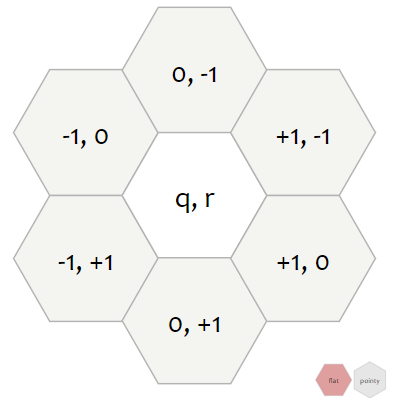
\includegraphics[width=0.5\textwidth]{coordiante.png}
        \caption{Voisins d'un hexagone}
        \end{figure}
    Où q et r sont les coordonnées axiales de l'hexagone.
    C'est aussi un système qui permet de facilement les tracer sur un écran.
    La formule de conversion des coordonnées axiales en coordonnées cartésiennes est la suivante :
    \begin{verbatim}
        x = size * (3./2 * q)
        y = size * (sqrt(3)/2 * q  +  sqrt(3) * r)
    \end{verbatim}
    Pour des illustrations détaillées de ce système nous vous renvoyons à \href{https://www.redblobgames.com/grids/hexagons/}{ce site qui nous a énormément aidé}.
    Nous définissons donc nos différents types concrets d'hexagones :
    \begin{itemize}
        \item \textbf{Place} : Les places du jeu, elles permettent d'avoir un multiplicateur de score.
        \item \textbf{Quarries} : Les carrières du jeu, elles permettent de gagner des ressources lorsqu'elles sont supperposées.
        \item \textbf{District} : Les quartiers du jeu, ils permettent de gagner des points de victoire.
    \end{itemize}
    La classe Hexagon et Tile implémentent toutes les deux serializable. Cela est dû au fait que nous voulious ajouter en extension un mode multijoueur en ligne.
    Cette fonctionnalité n'a pas été implémentée mais nous avons prévu le coup en rendant nos classes serializable (plus de détails dans la section \ref{subsec:extensions}).
    \subsection{Interface Graphique}\label{subsec:interface-graphique}

    Comme mentionné précédemment, l'interface graphique du jeu est réalisée en utilisant la bibliothèque Swing, qui permet de créer des interfaces graphiques en Java.
    L'avantage de son utilisation est qu'elle est incluse dans la bibliothèque standard de Java, ce qui signifie qu'elle est disponible sur toutes les plateformes Java.
    Nous allons expliquer le fonctionnement de Swing.
    \newline
    Swing utilise un modèle de composants légers, ce qui signifie que les composants Swing sont indépendants de la plateforme et ne dépendent pas des composants natifs de la plateforme.
    Cela signifie que les composants Swing ont un aspect et un comportement cohérents sur toutes les plateformes (sur le papier en tout cas mais en pratique c'est pas toujours le cas).
    C'est cela qui le différencie de AWT (Abstract Window Toolkit) qui utilise des composants lourds qui dépendent des composants natifs de la plateforme.
    Cela ne signifie pas que Swing ne peut pas utiliser les composants natifs de la plateforme, on peut toujours utiliser les composants AWT dans Swing.
    Par contre on ne peut pas utiliser les composants Swing dans une application AWT.
    Le JFrame est la fenêtre principale de l'application Swing. C'est la fenêtre qui contient tous les autres composants Swing.
    Les composants Swing sont des objets qui héritent de la classe JComponent.
    On peut ajouter des composants Swing à un JFrame en utilisant la méthode add() de la classe Container.
    Il y a pas mal de composants qui sont disponibles dans Swing, comme le JPanel pour regrouper nos composants, le JButton pour créer un bouton programmable ou encore le JLabel pour afficher du texte.
    \newline
    Tout le rendu graphique est géré par Swing dans un thread séparé appelé Event Dispatch Thread (EDT).
    Il est important de ne pas bloquer l'EDT avec des opérations longues, sinon l'interface graphique deviendra non réactive.
    Il est aussi impossible de modifier les composants Swing en dehors de l'EDT, Swing n'est pas thread-safe.
    Cela ne veut pas dire qu'on ne peut pas utiliser plusieurs threads dans une application Swing, mais il faut faire attention à ne pas modifier les composants Swing en dehors de l'EDT.
    Fort heureusement, Swing fournit des méthodes pour exécuter du code dans l'EDT, comme la méthode invokeLater() de la classe EventQueue.
    Il est également possible de créer des threads SwingWorker pour exécuter des tâches longues en arrière-plan sans bloquer l'EDT.
    Aussi il est tout à fait possible de créer ses propres composants Swing en étendant la classe JComponent ou une de ses sous-classes (comme JPanel).
    On peut alors redéfinir les méthodes paintComponent() et/ou paint() pour personnaliser le rendu du composant.
    C'est ce que nous avons fait pour la plupart des composants de notre jeu puisque la plupart des composants Swing manquent de fonctionnalités.
    Par exemple, le Jlabel ne permet pas d'avoir une bordure autour de notre texte, il a fallu créer notre propre composant pour cela.
    \newline
    Swing utilise la programmation événementielle pour gérer les interactions de l'utilisateur.
    Les composants Swing possèdent des écouteurs appelés EventListeners qui sont notifiés lorsqu'un événement que l'on souhaite écouter se produit.
    Les EventListeners sont des interfaces qui définissent des méthodes qui sont appelées lorsqu'un événement se produit.
    Les classes très utiles de Listeners sont les MouseListener qui permettent de gérer les événements de la souris (les clics, les déplacements, etc.) et les KeyListener qui permettent de gérer les événements du clavier (les touches pressées, relâchées, etc.).
    Il est également possible de créer ses propres écouteurs en implémentant les différentes interfaces de Listener.
    \newline
    Enfin, il existe des LayoutManagers qui permettent de gérer la disposition des composants dans une fenêtre.
    On peut sinon hardcoder la position des composants mais il faudra alors gérer les redimensionnements de la fenêtre.
    Si nous n'avons pas de LayoutManager, il faudra donc définir la taille et la position de chaque composant à la main sinon ils ne s'afficheront pas.
    Cela peut être très fastidieux et compliqué, c'est pourquoi il est recommandé d'utiliser un LayoutManager lorsque c'est possible.
    Le problème est que les LayoutManagers de Swing ne sont pas toujours très flexibles.
    Ils sont souvent soit trop rigides et simplistes, soit trop complexes et difficiles à utiliser.
    C'est pourquoi il est souvent nécessaire de combiner plusieurs LayoutManagers pour obtenir le résultat souhaité.
    \newline
    Le framework Swing est assez ancien : il date de 1997 et a été inclu dans la JDK 1.2.
    Les fonctionnalités sont limités : il n'y a qu'une classe de Timer pour gérer les animations, pas de support pour les shaders, pas de support direct pour les effets sonores, la 3D et pas de décodeur vidéo intégré.
    Ceci n'est pas aidé par l'existence d'autres frameworks plus modernes et plus flexibles comme JavaFX qui inclue un support pour les animations, les effets sonores, la 3D et les vidéos (pour les shaders il faudra passer par OpenGL par exemple).
    Cela dit, il est tout à fait possible de combiner Swing avec JavaFX pour profiter des avantages des deux frameworks.
    On peut aussi utiliser des bibliothèques tierces pour ajouter des fonctionnalités manquantes à Swing, ou même créer ses propres composants personnalisés.
    Notre interface reste assez simple à cause de ces limitations et de la non utilisation de frameworks tiers.


    \subsection{Extensions possibles}\label{subsec:extensions}

    Diverses extensions pour notre projet sont possibles. Nous avons déjà évoqué la possibilité d'ajouter un mode multijoueur en ligne.
    Nous avions réussi en local à envoyer des objets serializables (comme les tuiles) entre deux clients. L'idée était que un joueur était à la fois serveur et client.
    Il y avait donc un joueur qui lançait le serveur et un autre qui se connectait à ce serveur en utilisant son adresse IP.
    Pour envoyer des objets serializables, il suffisait d'utiliser un ObjectInputStream et un ObjectOutputStream sur les sockets.
    Grâce donc au protocole TCP, les objets étaient envoyés de manière fiable et ordonnée malgré la latence du réseau (ce qui en soit n'est pas un problème pour un jeu de société tour par tour).
    Pour pouvoir l'implémenter il faudrait principalement la partie graphique avec les listeners pour les désactiver lorsqu'on attend un message du serveur.
    En plus de cela, il faudrait faire attention à la synchronisation des threads pour éviter les problèmes de concurrence sans oublier de gérer les déconnexions.
    Cela aurait été une extension très intéressante mais qui demandait beaucoup de temps et de travail.
    \newline
    Une autre extension possible est l'ajout d'une intelligence artificielle pour jouer contre l'ordinateur.
    Cela aurait été une extension intéressante mais qui demandait également beaucoup de temps et de travail.
    La raison pour laquelle nous n'avons pas implémenté cette extension est que nous avons préféré nous concentrer sur la réalisation du jeu de base.
    De plus, Akropolis est un jeu de société complexe qui demande une réflexion stratégique importante.
    Pour avoir une intelligence artificielle capable de rivaliser avec un joueur humain, il aurait fallu une IA suffisament sophistiquée pour prendre en compte toutes les possibilités de jeu.
    La gestion de quoi choisir dans la pioche par exemple puisque l'on ne peut pas voir les tuiles suivantes il y a une part de hasard à moins de la faire tricher en regardant les tuiles suivantes.
    Ensuite de nombreux coups sont possibles et un coup qui peut sembler bon peut se révéler catastrophique plus tard.
    La gestion donc de la profondeur de recherche et de l'évaluation des coups possibles aurait été très complexe.
    Il faut avoir une IA capable de réaliser des coups aussi suffisament rapidement pour ne pas ennuyer le joueur donc il faudrait vraiment bien optimiser le modèle.
    Une variante du min max aurait été une solution mais encore faut-il avoir une fonction d'évaluation correcte.

    \section{Difficultés Rencontrées}\label{sec:difficultes-rencontrees}

    Dans un premier temps, une des plus grosse difficulté rencontrée a été de choisir une implémentation efficace, cohérente et en accord avec les règles et le fonctionnement du jeu.
    La principale difficulté était de trouver une bonne méthode afin de gérer les coordonnées des hexagones, en pensant également à l'implémentation futur de la vue.
    On a ainsi essayé ou pensé à plusieurs implémentations, une liste chainée, un tableau, une hashmap, etc.
    Durant les deux ou trois premières semaines, nous avons tourné en rond pour trouver une implémentation qui nous convenait.
    Après discussions, et après avoir demandé l'avis de notre encadrant de projet, nous avons finalement opté pour une implémentation sur une hashmap contenant des paires de coordonnées (Point3D) et de tuiles (Hexagon), pour ce qui est de la classe Point3D, elle étend une classe déjà existante; Point2D de Java.
    Et la classe Hexagon a été créer sur mesure pour ce projet.
    Dans le modèle une autre difficulté a été de calculer les scores puisque chaque quartier est régi par des règles de calcul spécifiques, avec plusieurs contraintes à respecter, comme le placement de la tuile, le type de la tuile, le nombre de tuiles supperposées, ect.
    Après avoir implémenté le modèle, nous avons décidé de nous attaquer à la vue, une autre très grande difficulté du projet pour plusieurs raisons, 
    la première étant que toute la gestion des coordonnées, que ce soient celles des hexagones, ou de la souris était d'une grande difficulté à implémenter pour facilité cette partie du travail nous sommes aller chercher des ressources sur internet et grâce \href{https://www.redblobgames.com/grids/hexagons/}{au site évoqué précédemment}.
    nous avons pu avoir une aide, surtout dans la gestion des formules pour adapter les coordonnées de la souris et des hexagones.
    Aussi le code graphique n'est pas optimisé. L'énorme majorité de la mémoire est utilisée par les HexagonOutlines qui sont des objets affichant juste une forme avec une bordure hexagonale.
    Ils sont créer en énorme quantité, un par hexagone donc en mode 4 joueurs ont atteint très facilement plus de 40 000 objets graphiques à afficher.
    Si l'on observe sur un outil de profiling comme VisualVM, on voit que la mémoire est utilisée à plus de 90\% par ces objets.
    Cela cause un léger temps de chargement au lancement d'une partie et une consommation de mémoire assez élevée puisqu'ils sont tous créer d'un coup même si ils ne sont pas encore visible.
    L'approche marche et le jeu ne rame pas mais il est clair que l'on pourrait optimiser cela. Une solution serait de recycler au maximum les objets graphiques en commun en les stockant dans un cache par exemple.
    Cela aurait rajouté de complexité au code, et puisque le jeu fonctionne correctement nous avons préféré ne pas le faire.
    La musique prend aussi beaucoup de mémoire car elle est en format wav non compressé.
    On ne pouvais pas la compresser en mp3 car la librairie Java Sound ne le supporte pas.

    \section{Conclusion}\label{sec:conclusion}

    \section{Annexes}\label{sec:annexes}



    \tableofcontents

\end{document}
